\documentclass[11pt, a4paper]{article}
\usepackage{fullpage}
\usepackage[USenglish]{babel}
\usepackage{graphicx} 
\usepackage[small,bf,hang]{caption2}
\usepackage{nameref}
\usepackage{hyperref}
\hypersetup{
    colorlinks,
    citecolor=black,
    filecolor=black,
    linkcolor=black,
    urlcolor=black
}

\title{Master Thesis -  Security Aspects in Virtual Networks\\ \textbf{SITREP 15}}
\author{\textbf{Laurent De Wilde} \\ Master of Science in the Applied Computer Science \\ Vrije Universiteit Brussel}
\date{April 9, 2015}

\begin{document}
\maketitle

\section*{Work done}

This is an overview of the work performed in the past day:
\begin{itemize}
\item Performed some benchmarking to compare the performances between encrypted and non-encrypted disks. Therefore, I used two different tools, to obtain more accurate results. The findings are listed below.
\end{itemize}
$\;$ \\ \\
\noindent\begin{minipage}{\textwidth}
    \centering
    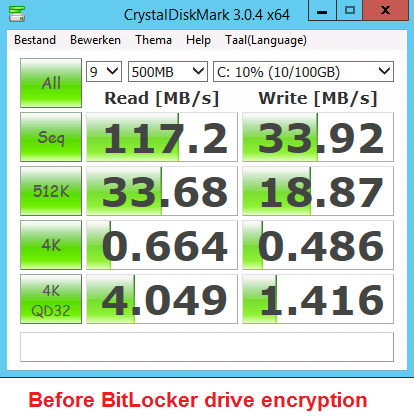
\includegraphics{Pre_BitLocker_1.png}
 \captionof{figure}{Read - and write speeds according to ``CrystalDiskMark'' before the drive has been encrypted by BitLocker. Note that I use an actual system (virtual) disk.}
\end{minipage}
$\;$ \\ \\
\noindent\begin{minipage}{\textwidth}
    \centering
    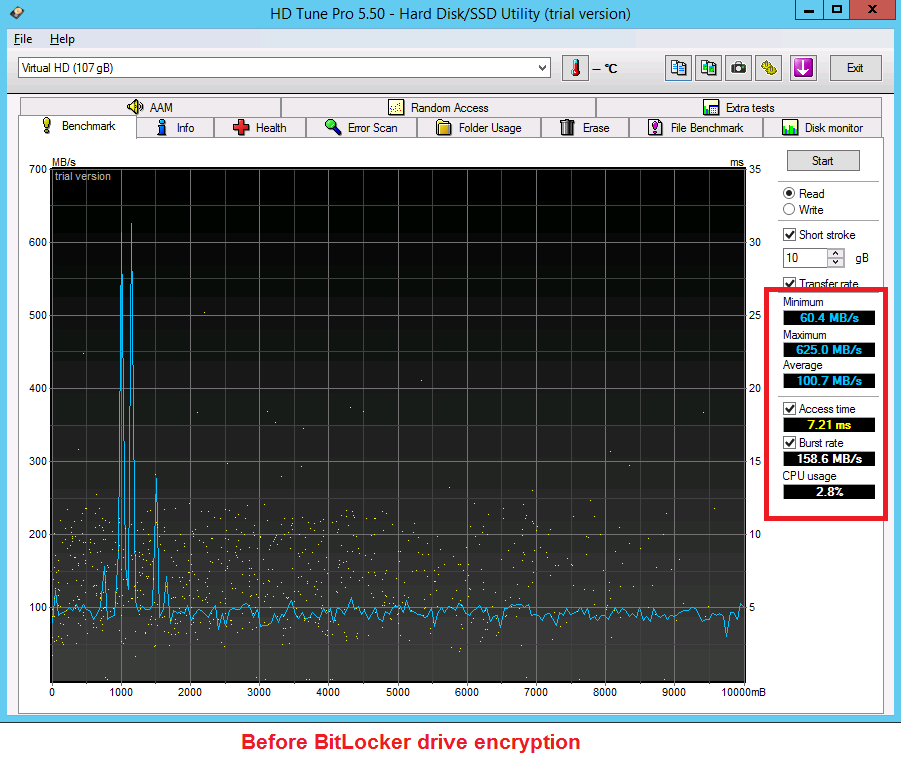
\includegraphics[width=\textwidth]{Pre_BitLocker_3.png}
 \captionof{figure}{Here I use HDTune Pro to perform the benchmarking.}
\end{minipage}
$\;$ \\ \\
\noindent\begin{minipage}{\textwidth}
    \centering
    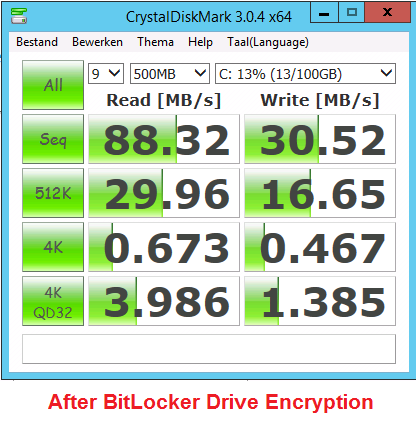
\includegraphics{Post_BitLocker_1.png}
 \captionof{figure}{These are the results after the system drive has been encrypted using BitLocker. The sequential read speed drops from 117 MB/s to 88 MB/s and the sequential write speed drops from 34 MB/s to 30 MB/s.}
\end{minipage}
$\;$ \\ \\
\noindent\begin{minipage}{\textwidth}
    \centering
    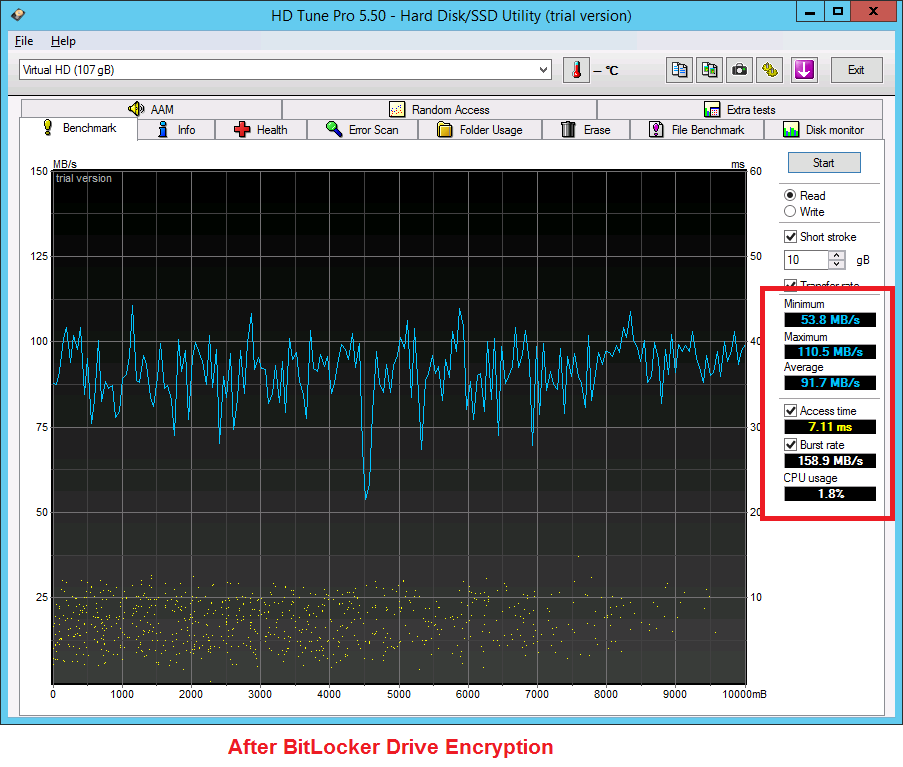
\includegraphics[width=\textwidth]{Post_BitLocker_2.png}
 \captionof{figure}{Also HDTune confirms the speed drop: from 100 MB/s on average to 91 MB/s on average.}
\end{minipage}
$\;$ \\ \\
Let us summarize the performance differences:
\begin{table}[h]
\begin{tabular}{|l|l|l|l|}
\hline
       & Before & After & Difference in \% \\ \hline
Read 1 & 117    & 88    & 24 \% slower     \\ \hline
Read 2 & 100    & 92    &   8 \% slower               \\ \hline
Write  & 34     & 30    &   12 \% slower               \\ \hline
\end{tabular}
\end{table}
$\;$ \\ \\
So in conclusion, if we take the average of the two reading speed differences, we can state that the reading speed is 16\% slower and the writing speed is 12\% slower. \\ \\
Note that the disk access time \textbf{remains the same} according to HDTune. The question now is: do we choose for performance but less security, or do we choose for security with a performance decrease of approximately 15\%?

\section*{Planning}



\section*{Problems}



\section*{Issues}
\label{sec:issues}
\noindent\begin{minipage}{\textwidth}
    \centering
    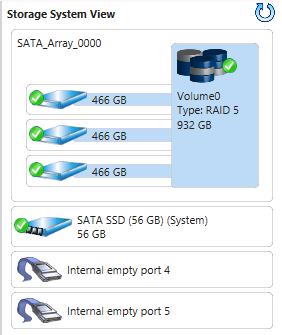
\includegraphics{RAID_1.png}
 \captionof{figure}{I have installed the Intel Rapid Storage Technology tool and this tool confirmes that all three the disks are working normally, despite the LED not blinking.}
\end{minipage}



\section*{Assistance}


\end{document}